\chapter{初等関数}
この章では,中学校・高等学校で学んだ\textbf{関数}について改めて定義を確かめ,その例である初等関数を個別に紹介する.

\section{関数とは}
数学における関数とは,ある集合から別の集合への対応関係を示したものである.イメージとして図\ref{fig:blackbox}のようなブラックボックス(中身が分からない箱)を思い浮かべるとよい.ここでは,改めて用語を定義し,数学における関数を形作っていきたい.

\vspace*{4cm}
\begin{figure}[!h]
	\caption{関数のイメージ}
	\label{fig:blackbox}
\end{figure}

\begin{definition}[集合] % set
	\textbf{集合}とは,ある対象(それは数であっても関数であっても,あるいは果物などであってもよい)を集めたものである.集合を構成する1つ1つの対象を\textbf{元}あるいは\textbf{要素}と呼ぶ.このとき,要素の順序や重複は気にしないものとする.また,対象が集合の要素であるかどうか真偽が決定できるように定義されなければならない.とくに,対象$a$が集合$A$の要素であるとき$a \in A$と表記し,要素でないとき$a \notin A$と表記する.
\end{definition}
\begin{rem*}
	$a \in A$の読み方としては,「$a$は$A$の要素である」以外にも「$a$は$A$に属している」「$A$は$a$を要素として持つ」などがある.
\end{rem*}
\begin{example*}
	$\set{1,2,3}$や$\set{\text{りんご}, \text{ばなな}, \text{みかん}}$は,集合の例である.このように具体的な要素を列挙することを,\ruby{{\textbf{外}}{\textbf{延}}}{がい|えん}記法という.また,$\set{x \mid x \text{は10以下の正の偶数}}$も集合の例である.このように集合に属する要素が満たすべき条件を明示することを,\ruby{{\textbf{内}}{\textbf{包}}}{ない|ほう}記法という.
\end{example*}
% % % 太字は,読者の目を止まらせるためのもの->ふりがなが重要でない場合には太字にしなくてもよい?
\begin{example*}
	$\set{1,1,3}$と$\set{1,3,1}$と$\set{1,3}$は,同一の集合である.そのため,通常は,最も少ない要素数になるように,特定の順序に従って表記される.
\end{example*}
\begin{example*}
	数の集合について,一般的に使われている記号を表\ref{table:number}に示す.これら数の集合のように,要素数が無限になる集合もあり,ほとんどの場合,内包記法によって表記される.
	\begin{table}[!h]
		\centering
		\caption{数の集合に用いられる記号}
		\label{table:number}
		\begin{tabular}{cc}
			$\mathbb{N}$ & 自然数全体の集合 \\
			$\mathbb{Z}$ & 整数全体の集合 \\
			$\mathbb{Q}$ & 有理数全体の集合 \\
			$\mathbb{R}$ & 実数全体の集合 \\
			$\mathbb{C}$ & 複素数全体の集合 \\
		\end{tabular}
	\end{table}
\end{example*}
\begin{definition}[空集合] % empty set
	集合において,要素が1つもない空っぽな集合を考えることができる.これを\textbf{空集合}といい,$\emptyset$と表記する.
\end{definition}
% % % 閉区間・開区間を,集合の例として紹介する?
% % % 開閉区間を取り入れるなら,上限・下限,最大・最小も取り入れたい.
% % % ->代数関数の項に移動

\begin{definition}[部分集合] % subset
	集合$X$が,集合$S$の\textbf{部分集合}であるとは,$X$の要素が全て$S$に属することである.このとき$X \subseteq S$と表記する.
\end{definition}
\begin{rem*}
	$X \subseteq S$の読み方としては,「$X$は$S$の部分集合である」以外にも「$X$は$S$に含まれる」「$S$は$X$を包含する」などがある.また,$X$が$S$の部分集合でない場合には,$X \nsubseteq S$と表記される.
\end{rem*}
\begin{example*}
	$\set{1,2,3}$は,自然数全体の集合$\mathbb{N}$の部分集合である.また,$\mathbb{N}$は,整数全体の集合$\mathbb{Z}$の部分集合である.
\end{example*}
\begin{example*}
	集合$S$について,空集合$\emptyset$と自分自身$S$は,常に部分集合である.
\end{example*}

複数の集合を用いて,新しい集合を作ることができる.ここでは,代表的なものを定義する.
\begin{definition}[和集合] % union, join
	\textbf{和集合}$A \cup B$とは,集合$A$と集合$B$に属する要素を集めた集合のことである.
\end{definition}
\begin{definition}[共通部分] % intersection
	\textbf{共通部分}$A \cap B$とは,集合$A$と集合$B$に\underline{同時に}属する要素を集めた集合のことである.
\end{definition}
\begin{rem*}
	$\cup$は「または」と読み,$\cap$は「かつ」と読む.
\end{rem*}
\begin{example*}
	集合$A=\set{1,2,3,4,5}$と集合$B=\set{3,4,5,6,7}$に対し,和集合$A \cup B$は$\set{1,2,3,4,5,6,7}$であり,共通部分$A \cap B$は$\set{3,4,5}$である.
\end{example*}

\begin{definition}[差集合] % set difference
	\textbf{差集合}$A \setminus B$とは,集合$A$に属する要素のうち,集合$B$に属していない要素を集めた集合のことである.
\end{definition}
\begin{example*}
	集合$A=\set{1,2,3,4,5}$と集合$B=\set{3,4,5,6,7}$に対し,差集合$A \setminus B$は$\set{1,2}$である.整数全体の集合$\mathbb{Z}$と集合$\set{0}$に対し,差集合$\mathbb{Z} \setminus \set{0}$は$\set{x \mid \text{$x$は正の整数または負の整数}}$である.
\end{example*}

ここまで定義した集合について,図示したものが図\ref{fig:VennDiagram}である.

\vfill
\begin{figure}[!h]
	\caption{集合の図示}
	\label{fig:VennDiagram}
\end{figure}
\clearpage

\begin{definition}[順序組] % ordered tuple, ordered list, ordered pair
	\textbf{順序組}とは,ある対象を集めたものである.このとき,集合とは違い,要素の順序や重複に意味があるものとする.
\end{definition}
\begin{example*}
	$(1, 2)$や$(\spadesuit, \text{K})$は,順序組の例である.このような2つの要素から成る順序組を\textbf{順序対}と呼ぶ.また,$(1, 2)$と$(2, 1)$は,異なる順序組であり,$(1, 1, 3)$と$(1, 3)$も異なる順序組である.
\end{example*}
\begin{definition}[直積集合] % (direct) product
	\textbf{直積集合}$A \times B$とは,集合$A$に属する要素と,集合$B$に属する要素から,新たに順序対を作り,それら全てを要素とする集合のことである.このとき,$A \times B$の要素である順序対$(a, b)$は,直積集合の表記通りの順序を保たなければならない.つまり,$a \in A, b \in B$である.
\end{definition}
\begin{example*}
	集合$A=\set{1,2,3}$と集合$B=\set{\heartsuit,\diamondsuit}$に対し,直積集合$A \times B$は$\set{(1, \heartsuit),(1,\diamondsuit),(2, \heartsuit),(2,\diamondsuit),(3, \heartsuit),(3,\diamondsuit)}$である.$(\heartsuit, 1)$など順序を逆にしたものは,$A \times B$の要素ではない.
\end{example*}
% % % 全体集合,補集合,対称差,冪集合,商集合は,今回の微積分に出てこないかも?のでカット

この直積集合を用いて,2つの集合間に二項関係を築くことができる.
\begin{definition}[二項関係] % binary relation
	\label{def:binaryRelation}%
	集合$A, B$間の\textbf{二項関係}$R$とは,直積集合$A \times B$の部分集合である.このとき,$R$の要素である順序対$(a,b)$を,$aRb$と表記することもある.また,集合$A$を\textbf{始集合}と呼び,集合$B$を\textbf{終集合}と呼ぶ.
\end{definition}
\begin{example*}
	集合$A=\set{1,2,3,4,5}$と集合$B=\set{3,4,5,6,7}$に対し,$aRb$を$a$は$b$を割り切る関係とする.このとき,関係$R$は,
	\[
		\set{(1,3),(1,4),(1,5),(1,6),(1,7),(2,4),(2,6),(3,3),(3,6),(4,4),(5,5)}
	\]
	である.
\end{example*}
% % % 反射的,対称的,推移的,同値関係
% % % 単射,全射,全単射
% % % 二項関係は,二項演算を含み,二項演算と二項算法はニアイコールである.

% 通常,二項関係は,様々な例を作ることができる.ここに一定の制約を加えることにより,写像を定義することができるようになる.
また,集合$A, B$間の二項関係$R$について,一定の条件を満たすことで,性質が定義される.
\begin{definition}[一意性]
	\label{def:uniqueness}
	\begin{align*}
	\text{$R$は単射(左一意的)である.} &\Leftrightarrow \text{集合$B$の要素$b$に対し,$aRb$が存在するならば,} \\
	&\qquad \text{$a$は一意的に決定できる.} \\
	\text{$R$は関数的(右一意的)である.} &\Leftrightarrow \text{集合$A$の要素$a$に対し,$aRb$が存在するならば,} \\
	&\qquad \text{$b$は一意的に決定できる.} \\
	\text{$R$は一対一である.} &\Leftrightarrow \text{$R$は左一意的かつ右一意的である.}
	\end{align*}
\end{definition}
\begin{definition}[全域性]
	\label{def:total}
	\begin{align*}
	\text{$R$は全域的(左全域的)である.} &\Leftrightarrow \text{集合$A$の要素$a$に対し,集合$B$の要素$b$が存在して,} \\
	&\qquad \text{二項関係$R$は$aRb$を要素として持つ.} \\
	\text{$R$は全射(右全域的)である.} &\Leftrightarrow \text{集合$B$の要素$b$に対し,集合$A$の要素$a$が存在して,} \\
	&\qquad \text{二項関係$R$は$aRb$を要素として持つ.} \\
	\text{$R$は対応である.} &\Leftrightarrow \text{$R$は左全域的かつ右全域的である.}
	\end{align*}
\end{definition}
\begin{definition}[写像および全単射]
	\label{def:specialRelations}
	\begin{align*}
	\text{$R$は写像(一意対応)である.} &\Leftrightarrow \text{$R$は関数的(右一意的)かつ全域的(左全域的)である.} \\
	\text{$R$は全単射(双射)である.} &\Leftrightarrow \text{$R$は単射かつ全射である.}
	\end{align*}
\end{definition}
\begin{comment}
\begin{definition}[一意性]
	\begin{align*}
		\text{$R$は単射(左一意的)である.} &\Leftrightarrow \forall a_1, a_2 \in A, \forall b \in B \left[a_1Rb \wedge a_2Rb \Rightarrow a_1 = a_2 \right] \\
		\text{$R$は関数的(右一意的)である.} &\Leftrightarrow \forall a \in A, \forall b_1, b_2 \in B \left[aRb_1 \wedge aRb_2 \Rightarrow b_1 = b_2 \right] \\
		\text{$R$は一対一である.} &\Leftrightarrow \text{$R$は左一意的かつ右一意的である.}
	\end{align*}
\end{definition}
\begin{definition}[全域性]
	\begin{align*}
	\text{$R$は全域射(左全域的)である.} &\Leftrightarrow \forall a \in A, \exists b \in B \text{ s.t. } aRb \\
	\text{$R$は全射(右全域的)である.} &\Leftrightarrow \forall b \in B, \exists a \in A \text{ s.t. } aRb \\
	\text{$R$は対応である.} &\Leftrightarrow \text{$R$は左全域的かつ右全域的である.}
	\end{align*}
\end{definition}
\end{comment}
定義\ref{def:uniqueness}と定義\ref{def:total}の一部を図示したものが,図\ref{fig:relationProperty}である.

\vfill
\begin{figure}[!h]
	\caption{定義\ref{def:uniqueness}と定義\ref{def:total}の図示}
	\label{fig:relationProperty}
\end{figure}
\afterpage{\clearpage}
\newpage

定義\ref{def:specialRelations}における写像の定義を言い換えたものが,定義\ref{def:mapping}である.
\begin{definition}[写像] % mapping, map
	\label{def:mapping}%
	\textbf{写像}$f$とは,始集合$A$と終集合$B$との間の関係$R$であり,始集合の要素$a$について,一意的に$aRb$が決定できるものである.
\end{definition}
\begin{definition}[関数] % function
	\textbf{関数}$f$とは,終集合が数の集合であるような写像のことである.
\end{definition}
% % % 独立変数,従属変数
% % % cod(f) = R -> 実数値関数
% % % dom(f) = cod(f) = R -> 実関数
% % % cod(f) = C -> 複素数値関数
% % % dom(f) = cod(f) = C -> 複素関数
\begin{rem*}
	写像あるいは関数$f$は,始集合$A$と終集合$B$を伴って$f : A \rightarrow B$と表記される.また,始集合のことを\textbf{始域}と呼び$\dom f$と表記する.同様に,終集合のことを\textbf{終域}と呼び$\cod f$と表記する.これは,誤解を恐れずに言うならば方言のようなものである(発展するに当たって歴史的背景が異なる分野において,同じ意味を表す異なる単語があることは不思議ではない).
\end{rem*}
% % % dom(f)もcod(f)もfが主語であり,関数全体の集合でどうこうを考えるためか?
% % % 始集合,終集合は,いずれも集合と名前がついている通り集合論の話っぽい
% % % 始域,終域は,それに対して写像,つまりマッピングのイメージに近い
\begin{rem*}
	写像あるいは関数$f$について,特に要素の関係を強調する場合には,$f : a \mapsto b$と表記される.$f$は関係であるため,要素として順序対$(a,b)$を持つ.これを,$afb$と表記しても良いが,一般的に$f(a) = b$と表記する.この$a$に対して,$b$が$f$によって指定されることを,「$a$が$f$によって$b$に写される」といい,$b$のことを$a$における$f$の\textbf{値}と呼ぶ.
\end{rem*}
% % % 始集合,initial set, source
% % % 始域,domain
% % % 定義域,domain of definition
% % % 終集合,target set, target
% % % 終域,codomain
% % % 値域,range
% % % 像,image
% % % 始集合と始域,終集合と終域は,同じ意味の語彙である.対して,定義域は始域の部分集合として,像は終域の部分集合である.値域は像の言い換えである場合がほとんどだが,文献によっては終域の意味の場合もある.
% % % image <= range <= codomain
% % % また,domainと書かれている場合,ほとんど定義域の意味で書かれていることが多い.写像の場合は,始域と定義域は等しいので,ほとんど区別されない.
% % % 像については,元の像,部分集合の像,写像の像と3種類の意味がある.元の像については,値(value)と呼ばれることもある.
\begin{example*}
	関数$f : \mathbb{R} \rightarrow \mathbb{R}; a \mapsto a^2$について,始域と終域はともに実数全体の集合$\mathbb{R}$である.また,$2$における$f$の値は,$4$である.つまり,$f(2) = 4$である.
\end{example*}

\begin{definition}[像]
	写像あるいは関数$f$について,その\textbf{像}$\im f$とは,始域の要素に対する$f$の値を集めた集合のことである.像は,終域の部分集合である.
\end{definition}
\begin{rem*}
	意味合いが似てるものに,値域と呼ばれる語句があるが,ほとんどの場合,像と同じ意味である.また,定義域と呼ばれる語句は,本来,始域の部分集合であるが,写像の場合は,始域と定義域は等しいので,ほとんど同一視されている.
\end{rem*}
\begin{example*}
	関数$f : \mathbb{R} \rightarrow \mathbb{R}; a \mapsto a^2$について,像$\im f$は,正の実数全体の集合$\mathbb{R}_{\geq 0}$である.
\end{example*}

\newpage
\section{代数関数}
% % % 押さえたい内容
% % % n次関数,因数定理,因数分解,解と係数の関係,複素共役,平方完成,関数のグラフの平行移動,簡単なグラフの概形
% % % 閉区間・開区間と,2次不等式
代数関数とは,関数の中でも特に,始域の要素$a$と終域の要素$b$とを結びつける二項関係が,ある\textbf{代数式}(多項式や有理式,無理式の総称)によって定義される関数のことを指す.
代数式の例を,表\ref{table:algebraicExpression}に示す.ここで,$x$は,単なる記号であり,これを\textbf{不定元}と呼ぶ.
% % % 係数,項,項の次数,多項式の次数,モニック(単多項式),定数項
% % % 因数,既約多項式
% % % 変数,不定元
% % % 式の値,恒等式,方程式

\begin{table}[!h]
	\centering
	\caption{代数式}
	\label{table:algebraicExpression}
	\begin{tabular}{cccc|c}
		& & & & 例 \\
		\hline
		\multirow{6}{*}{代数式} & & \multirow{4}{*}{多項式} & 定数式 & $3$ \\
		& & & 一次式 & $2x+1$ \\
		& 有理式& & 二次式 & $3x^2+x+2$ \\
		& & & n次式 & $\sum_{i=0}^{n}a_ix^i\quad(a_n \neq 0)$ \\
		\cline{3-5}
		& & 分数式 & & $6/x, (2x+1)/(3x^2+x+2)$ \\
		\cline{2-5}
		& 無理式 & & & $\sqrt{x}, x^{2/3}$ \\
	\end{tabular}
\end{table}

\begin{comment}
\begin{table}[!h]
	\centering
	\caption{代数式}
	%\label{table:algebraicExpression}
	\[
		\text{代数式}
		\begin{cases}
			\text{有理式}
			\begin{cases}
				\text{多項式} 
				\begin{cases}
					\text{定数式} & 3, c\\
					\text{一次式} & ax+b \\
					\text{二次式} & ax^2+bx+c \\
					\text{$n$次式} & \sum_{i=0}^{n}a_ix^i
				\end{cases} \\
				\text{分数式} & \hspace*{-23mm}a/x
			\end{cases} \\
			\text{無理式} & \hspace*{-10mm}\sqrt{x}
		\end{cases}
	\]
\end{table}
\end{comment}

この節では,まず,多項式の因数定理を学ぶ.因数定理は,高次の多項式を,低次の多項式の積へと分解するために必要な因数を教えてくれる定理である.これから先,代数関数の積分を計算する際に,使用する定理なので,いくつかの計算練習も行う.
また,方程式や不等式について復習し.グラフとの関係について取り上げる.

\begin{comment}
\begin{definition}[二次式]
	$x$を不定元,$a, b, c$を定数とし,特に$a \neq 0$とする.このとき$ax^2+bx+c$で表現される多項式を,二次式と呼ぶ.
\end{definition}
\end{comment}
\begin{definition}[代入]
	代数式$P\langle x\rangle$に対し,不定元$x$を,異なる不定元あるいは集合$S$の要素$a$に置き換えることを\textbf{代入}と呼ぶ.$a$を代入することによって得られる$P\langle a\rangle$のことを,$a$において\textbf{評価}した値,あるいは\textbf{式の値}と呼ぶ.
\end{definition}
\begin{definition}[根]
	$P\langle x\rangle$を多項式とする.$P\langle x\rangle$に代入したとき,式の値が$0$となるような$a$のことを,多項式の\textbf{根}と呼ぶ.
\end{definition}
\begin{example*}
	二次式の根を求める方法の1つに,因数分解を利用する方法がある.代表的な二次式の因数分解の公式に
	\[
		x^2-(\alpha+\beta)x+\alpha\beta = (x-\alpha)(x-\beta)
	\]
	があり,このように因数分解できる場合,根は$\alpha, \beta$である.
\end{example*}
\begin{example*}
	二次式$x^2-5x+6$は,$(x-2)(x-3)$と因数分解できるため,この二次式の根は,$2, 3$である.また,二次式$x^2+2x+1$は,$(x+1)^2$と因数分解できる.これは,$(x+1)(x+1)$をまとめて表記したものであるため,$x^2+2x+1$の根は,$-1, -1$である.ただし,いくつかの根のうち等しい値がある場合,それらは等しい値ごとにまとめて書くため,この場合は$-1\,\text{(\textbf{重根})}$と表記される.
\end{example*}
\begin{theorem}[因数定理]
	多項式$P\langle x\rangle$の根の1つを$a$と置く.このとき,$P\langle x\rangle$は$(x-a)$を因数に持ち,$P\langle x\rangle = (x-a)Q\langle x\rangle$と表現することができる.ここで$Q\langle x\rangle$は,$P\langle x\rangle$の次数より1つ低い次数を持つ多項式である.
\end{theorem}
\begin{rem*}
	この定理の主張は,ある多項式$P\langle x\rangle$について,$a$を代入したとき,式の値$P\langle a\rangle$が$0$になるならば,$P\langle x\rangle$は$(x-a)$で割り切れる,ということである.手計算の際には,$0, 1, -1$など小さい値から順に代入していき,式の値が$0$になった数を使って,多項式の割り算を行うという手順を踏むことになる.
\end{rem*}
\begin{example*}
	多項式$P\langle x\rangle = x^3+x^2-x-1$は,$x = 1$を代入すると,$P\langle 1\rangle = 0$となる.つまり,この多項式の根の1つが$1$であることが分かる.よって,多項式$P\langle x\rangle$は,$(x-1)$を因数に持つため,これで割ることができ,$P\langle x\rangle = (x-1)(x^2+2x+1)$となる.したがって,多項式$P\langle x\rangle$を因数分解すると,$(x-1)(x+1)^2$となり,$P\langle x\rangle$の根は,$1, -1\,\text{(重根)}$であることが分かる.
\end{example*}
% % % 練習問題を別途作成する.

\begin{theorem}
	$a_i\quad(0 \leq i \leq n)$は,整数であり,特に,$a_n, a_0$は$0$でない整数とする.
	多項式$P\langle x\rangle$を,$P\langle x\rangle = a_nx^n+a_{n-1}x^{n-1}+\cdots+a_1x+a_0$とおく.
	このとき,$P\langle x\rangle$の根が,有理数$r$であるならば,
	\[
	r = \frac{\text{$a_0$の約数}}{\text{$a_n$の約数}}
	\]
	と書くことができる.
\end{theorem}
% % % 約数の定義をしていないが,整数の約数を,プラスマイナス含めたものにする
\begin{rem*}
	この定理は,整数係数の多項式を,因数定理を用いて因数分解する場合に有効である.
	言い換えれば,多項式の根となり得る候補を絞るための定理であるため,候補全てが根とならなかった場合,その多項式は,無理数根か,複素数根しか取らないことが分かる.
\end{rem*}
% % % モニックな整数係数多項式において,整数根を持たないならば有理数根を持たない
\begin{theorem}[アイゼンシュタインの既約判定定理]
	$a_i\quad(0 \leq i \leq n)$は,整数であり,特に,$a_n, a_0$は$0$でない整数とする.
	多項式$P\langle x\rangle$を,$P\langle x\rangle = a_nx^n+a_{n-1}x^{n-1}+\cdots+a_1x+a_0$とおく.
	ある素数$p$が存在し,以下の条件を満たすならば,有理数係数の範囲で因数分解したとき,$P\langle x\rangle$は,$k$次式以上の多項式を因数に持つ.
	\begin{itemize}
		\item $a_0$は,$p$の倍数だが,$p^2$の倍数でない.
		\item $a_i\quad(1 \leq i \leq k-1)$は,全て$p$の倍数である.
		\item $a_k$は,$p$の倍数でない.
	\end{itemize}

	特に,$k = n$の場合,$P\langle x\rangle$は,それ以上有理数係数の範囲で因数分解できない既約な多項式である.
\end{theorem}
% % % 整数係数の範囲で既約であれば,有理数係数の範囲でも既約である.
\begin{rem*}
	この定理は,十分条件であるため,有理数係数の範囲で既約な多項式だからといって,条件を満たすような素数$p$があるとは限らない.例えば,$x^2+5x+2$は,有理数係数の範囲で既約であるが,条件を満たすような素数は存在しない.
\end{rem*}
\begin{example*}
	多項式$x^2+2x+6$について,$p = 2$とする.$a_0 = 6$は,$p$の倍数かつ$p^2$の倍数でない.$a_1 = 2$は,$p$の倍数である.$a_2 = 1$は,$p$の倍数でない.よって,アイゼンシュタインの既約判定定理より,この多項式は,有理数係数の範囲で既約である.
\end{example*}

\begin{definition}[恒等式]
	$P\langle x\rangle, Q\langle x\rangle$を代数式とする.集合$S$における,すべての要素$a$に対して,$P\langle a\rangle = Q\langle a\rangle$が成り立つとき,これを\textbf{恒等式}と呼ぶ.
\end{definition}
\begin{definition}[方程式]
	$P\langle x\rangle, Q\langle x\rangle$を代数式とする.集合$S$における,ある要素$a$に対して,$P\langle a\rangle = Q\langle a\rangle$が成り立つかどうか真偽が決定できるとき,これを\textbf{方程式}と呼ぶ.また,等号が成り立つような$a$のことを\textbf{解}と呼ぶ.
\end{definition}
\begin{definition}[不等式]
	$P\langle x\rangle, Q\langle x\rangle$を代数式とする.また演算$\star$を$<, \leq, >, \geq$のいずれかと決める.集合$S$における,ある要素$a$に対して,$P\langle a\rangle \star Q\langle a\rangle$が成り立つかどうか真偽が決定できるとき,これを\textbf{不等式}と呼ぶ.また,不等号が成り立つような$a$のことを\textbf{解}と呼ぶ.
\end{definition}
\begin{rem*}
	方程式や不等式は,解が複数あることがほとんどである.そのため,すべての解を要素として持つ集合を\textbf{解集合}と呼び,解集合を求めることを,方程式あるいは不等式を\textbf{解く},という\footnotemark[2].また,解集合のことを,そのまま解と呼ぶこともある.
\end{rem*}
\footnotetext[2]{当然,解が存在しない場合も考えられ,その場合の解集合は,空集合$\emptyset$である.}
\begin{definition}[閉区間・開区間]
	ある実数$a, b$について(ただし$a \leq b$),\textbf{閉区間}$\left[a, b\right]$とは,$\set{x \mid a \leq x \leq b}$となる集合のことである.また,\textbf{開区間}$\left(a, b\right)$とは,$\set{x \mid a < x < b}$となる集合のことである.不等号の組み合わせによって,$\left[a, b\right) = \set{x \mid a \leq x < b}$と$\left(a, b\right] = \set{x \mid a < x \leq b}$も定義される.
\end{definition}
\begin{rem*}
	$\left(a, b\right)$と書かれている場合,文脈から開区間なのか順序対なのか判断する必要がある.また,閉区間・開区間については,数直線上に描くことができ,図\ref{fig:interval}のようになる.特に,ある実数$c$よりも小さい数の集合を,$\left(-\infty, c\right)$と表記したり,ある実数$c$以上の数の集合を$\left[c, \infty\right)$と表記したりする.
	
	\vfill
	\begin{figure}[!h]
		\caption{閉区間と開区間の図示}
		\label{fig:interval}
	\end{figure}
\end{rem*}
% % % \infty は通常,実数には含まれないが,ここではあえて触れないことにする.
\clearpage

\begin{definition}[多項式関数のグラフ]
	\label{def:graphPolynomial}%
	ある多項式$P\langle X\rangle$が与えられているとき,関数$f : \mathbb{R} \rightarrow \mathbb{R}; x \mapsto P\langle x\rangle$の\textbf{グラフ}とは,$f$の要素である順序対$(x, P\langle x\rangle)$を,$xy$平面上の点として描いたものである.
	このとき$x$は,始域$\mathbb{R}$の全ての要素となり得るので,\textbf{変数}あるいは未知数と呼ばれる.
	通常は,$x$における$f$の値を$y$と置き,$y = f(x)$と表記する.$x$における$f$の値は,$P\langle x\rangle$であるため,これを用いて$y = P\langle x\rangle$や$f(x) = P\langle x\rangle$と表記することもある.
\end{definition}
% % % 分数関数は,分母のゼロ割りが発生しないように定義域を変更する必要があり,無理関数も,根号の中身が負にならないように,定義域を変更する必要がある.
\begin{rem*}
	多項式$P\langle x\rangle$と多項式関数$f(x)$の違いは,単なる記号である$x$か,何らかの要素を取り得る変数としての$x$かの違いである.そのため,定義\ref{def:graphPolynomial}では,単なる記号であることを強調するため,多項式の不定元に$X$を用いた.
\end{rem*}
% % % 変数は,要素が固定である定数に対する,用語であり,要素が変化することが期待されている.
% % % 変数が取り得る要素の集合を,変域あるいは定義域と呼ぶ.
% % % 関数の文脈において,変数とは「関数の引数となるべき何らかの集合の元を代表するもの」である.

\begin{example*}
	多項式$x-2$と$2x-3$について,$x = 1$を代入すると,お互いの式の値が$-1$となり等しくなる.つまり,方程式$x-2 = 2x-3$の解は,$x = 1$である\footnotemark[3].これは,一次関数$y = x-2$と$y = 2x-3$の交点$(1, -1)$に対応する.
\end{example*}
\begin{example*}
	方程式$x^2-5x+6 = x-2$の解は,$x = 2, 4$である\footnotemark[3].これは,二次関数$y = x^2-5x+6$と一次関数$y = x-2$の交点$(2, 0), (4, 2)$に対応する.
\end{example*}
\footnotetext[3]{解集合という意味での解であれば$x = \set{1}$あるいは$x = \set{2,4}$と書かなければならない.ここでは,等号が成り立つ要素としての解であり,$x = 2,4$と書いてある場合は,「解は,$2$または$4$」と読む.}
\begin{example*}
	不等式$x^2-5x+6 \leq x-2$の解は,$2 \leq x \leq 4$である.これは,二次関数$y = x^2-5x+6$よりも一次関数$y = x-2$のほうが大きくなるか等しくなる$x$の区間が,$\left[2, 4\right]$であることに対応する.同様に,不等式$x^2-5x+6 > x-2$の解は,$x < 2,\; 4 < x$である.これは,二次関数$y = x^2-5x+6$よりも一次関数$y = x-2$のほうが小さくなる$x$の区間が,$\left(-\infty, 2\right) \cup \left(4, \infty\right)$であることに対応する.
\end{example*}

ここまでの例について,図示したものが図\ref{fig:equation}である.

\vfill
\begin{figure}[!h]
	\caption{方程式の解,不等式の解とグラフとの関係の図示}
	\label{fig:equation}
\end{figure}
\clearpage

% % % 解と係数の関係,複素共役 -> 計算上のテクニックになるので,とりあえず一旦保留.というか代数学の話では??
% % % 平方完成,関数のグラフの平行移動,簡単なグラフの概形
ここまでで,二次関数のグラフと,二次方程式あるいは二次不等式の解との関係を見てきた.
グラフを図示することにより,代数的な解と,幾何的な交点の$x$座標が同一視できることが分かる.
このように,グラフの図示,つまり関数の可視化は,関数の気持ちを理解する上でかかせないポイントであるため,ここでは,二次関数のグラフを描く際に使われる平方完成という手法を紹介する.平方完成は,二次関数のグラフを描くためだけではなく,代数関数の積分においても重要な役割を果たす計算手法である.

\begin{definition}[平方完成]
	二次式$ax^2+bx+c$について,$a(x-p)^2+q$の形に変形することを\textbf{平方完成}と呼ぶ.
\end{definition}
% % % 一般形 : ax^2+bx+c
% % % 標準形 : a(x-p)^2+q
% % % (因数)分解形 : a(x-s)(x-t)
\begin{algorithm}
	\begin{align}
		ax^2+bx+c &= a\left(x^2+\frac{b}{a}x\right)+c \tag{1} \\
		&= a\left\{\left(x+\frac{b}{2a}\right)^2-\frac{b^2}{4a^2}\right\}+c \tag{2} \\
		&= a\left(x+\frac{b}{2a}\right)^2-\frac{b^2}{4a}+c \tag{3} \\
		&= a\left(x+\frac{b}{2a}\right)^2-\frac{b^2-4ac}{4a} \tag{4}
	\end{align}
	
	各計算ステップは,以下の通りである.
	\begin{enumerate}[(1)]
		\item $ax^2+bx$について$a$でくくる.
		\item $x^2+\frac{b}{a}x$を変形する.ここでは,$\left(x+\frac{b}{2a}\right)^2$を展開することによって,$x^2+\frac{b}{a}x+\frac{b^2}{4a^2}$となるので,余分な$\frac{b^2}{4a^2}$を引くことによって,$x^2+\frac{b}{a}x$を作っている.
		\item $a$を$\left(x+\frac{b}{2a}\right)^2$と$-\frac{b^2}{4a^2}$に,分配する.
		\item $-\frac{b^2}{4a}$と$c$を通分する.
	\end{enumerate}

	結果として
	\begin{empheq}[left=\empheqlbrace]{align*}
		p &= -\frac{b}{2a} \\
		q &= -\frac{b^2-4ac}{4a}
	\end{empheq}
	を得る.
\end{algorithm}
\begin{rem*}
	二次関数$y = f(x) = a(x-p)^2+q$は,$x = p$のとき,$a$の符号によって,最大値あるいは最小値として$y = q$をとる.この,二次関数の最大値あるいは最小値を決める点$(p, q)$を,\textbf{頂点}と呼ぶ.
\end{rem*}
\begin{example*}
	二次式$x^2-5x+6$は,$\left(x-\frac{5}{2}\right)^2-\frac{1}{4}$と平方完成できるため,二次関数$f(x) = x^2-5x+6$は,頂点$\left(\frac{5}{2}, -\frac{1}{4}\right)$を通るグラフである.また,この関数の像$\im f$は,区間$\left[-\frac{1}{4}, \infty\right)$である.
\end{example*}

\begin{definition}[グラフの平行移動]
	多項式関数$f(x)$が与えられているとき,新たに多項式関数$g(x) = f(x-p) + q$を作ることができる.このとき,$g(x)$のグラフは,$f(x)$のグラフを$x$軸方向に$p$,$y$軸方向に$q$だけ動かしたものであり,これをグラフの\textbf{平行移動}という.
\end{definition}
\begin{example*}
	関数$f(x) = x^2$とすると,関数$g(x) = x^2-5x+6$は,$g(x) = \left(x-\frac{5}{2}\right)^2-\frac{1}{4} = f\left(x-\frac{5}{2}\right)-\frac{1}{4}$と書くことができる.したがって,$g(x) = x^2-5x+6$のグラフは,$f(x) = x^2$のグラフを,$x$軸方向に$\frac{5}{2}$,$y$軸方向に$-\frac{1}{4}$だけ動かしたものである.
\end{example*}

ここまでの例について,図示したものが図\ref{fig:quadraticFunction}である.

\vfill
\begin{figure}[!h]
	\centering
	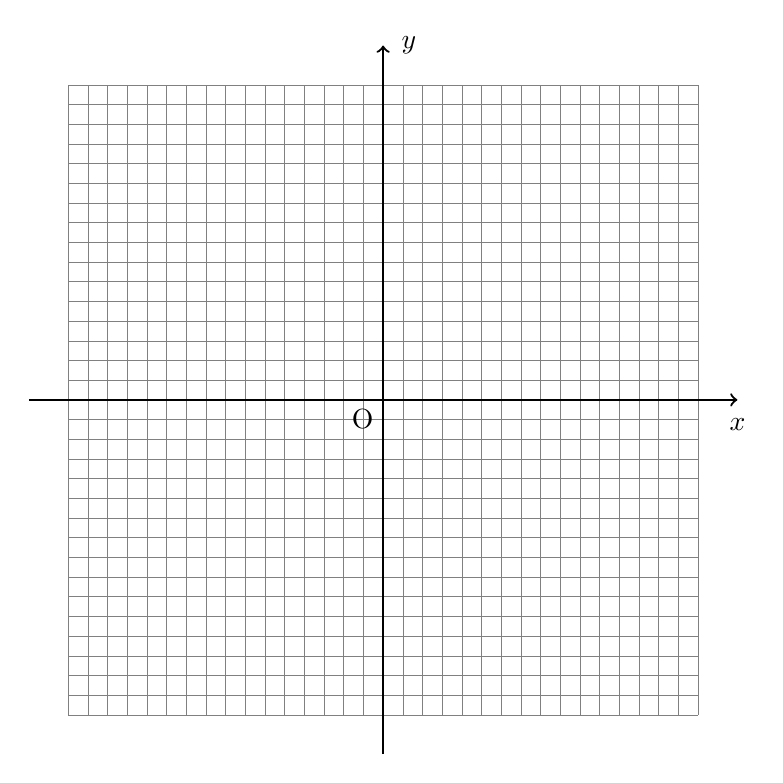
\begin{tikzpicture}
		\draw[help lines, step=0.25] (0,0) grid (8,8);
		\draw (4,4) node[below left]{O};
		\draw[thick, ->] (-0.5,4)--(8.5,4) node[below=3.0] {$x$};
		\draw[thick, ->] (4,-0.5)--(4,8.5) node[right=3.0] {$y$};
	\end{tikzpicture}
	\caption{二次関数のグラフの図示}
	\label{fig:quadraticFunction}
\end{figure}
\clearpage

\begin{definition}[分数関数のグラフ]
	ある多項式$P\langle X\rangle, Q\langle X\rangle$が与えられているとき,分数式$R\langle X\rangle$は,$R\langle X\rangle = P\langle X\rangle/Q\langle X\rangle$と表現することができる.
	関数$f : \mathbb{R}\setminus\set{a \mid a\text{は$Q\langle X\rangle$の根}} \rightarrow \mathbb{R}; x \mapsto R\langle x\rangle$のグラフとは,$f$の要素である順序対$(x, R\langle x\rangle)$を,$xy$平面上の点として描いたものである.
\end{definition}
\begin{example*}
	分数関数$f(x) = (x-2)/(x^2-6x+8)$は,$x = 2, 4$において値が定義されない.しかし,$x^2-6x+8 = (x-2)(x-4)$と因数分解することにより,分数式$(x-2)/(x^2-6x+8)$と分数式$1/(x-4)$は,$\mathbb{R}\setminus\set{2,4}$において,恒等式となる.ここで,分数関数$g(x) = 1/(x-4)$は,集合$\mathbb{R}\setminus\set{4}$において定義されているため,$f(2) = g(2) = -1/2$と値を定義することによって,分数関数$f(x)$と$g(x)$は,同一視できる.
\end{example*}
\begin{rem*}
	計算上,分数関数を考える場合,値を再定義するという回りくどいことは,ほとんど行われない.すでに見たように,分母を因数分解することによって,多項式の約分を行うことができるため,それ以上約分できない既約な分数式で表現される分数関数の形に変形し,計算を行っていく.
\end{rem*}
\begin{definition}[無理関数のグラフ]
	ある無理式$P\langle X\rangle$が与えられているとき,関数
	\[
	f : \set{x \mid \text{各項の値が実数になる$x$の区間の共通部分}} \rightarrow \mathbb{R}; x \mapsto P\langle x\rangle
	\]
	のグラフとは,$f$の要素である順序対$(x, P\langle x\rangle)$を,$xy$平面上の点として描いたものである.
\end{definition}
% % % 無理式と冪根を結びつける.特に,$x$の有理数乗が,$x$の冪根の累乗と定義されることを示しておくことで,指数関数に入りやすくなる?
\begin{example*}
	無理関数$f(x) = \sqrt{x}$は,区間$\left[0, \infty\right)$において,実数の値をとる.また,無理関数$g(x) = \sqrt{x-2}-1$は,区間$\left[2, \infty\right)$において,実数の値をとる.実数値関数において,根号内は負数にしない,ということに気をつけて,区間を選ぶ必要がある.
\end{example*}

ここまでの例について,図示したものが図\ref{fig:algebraicFunction}である.

\vfill
\begin{figure}[!h]
	\centering
	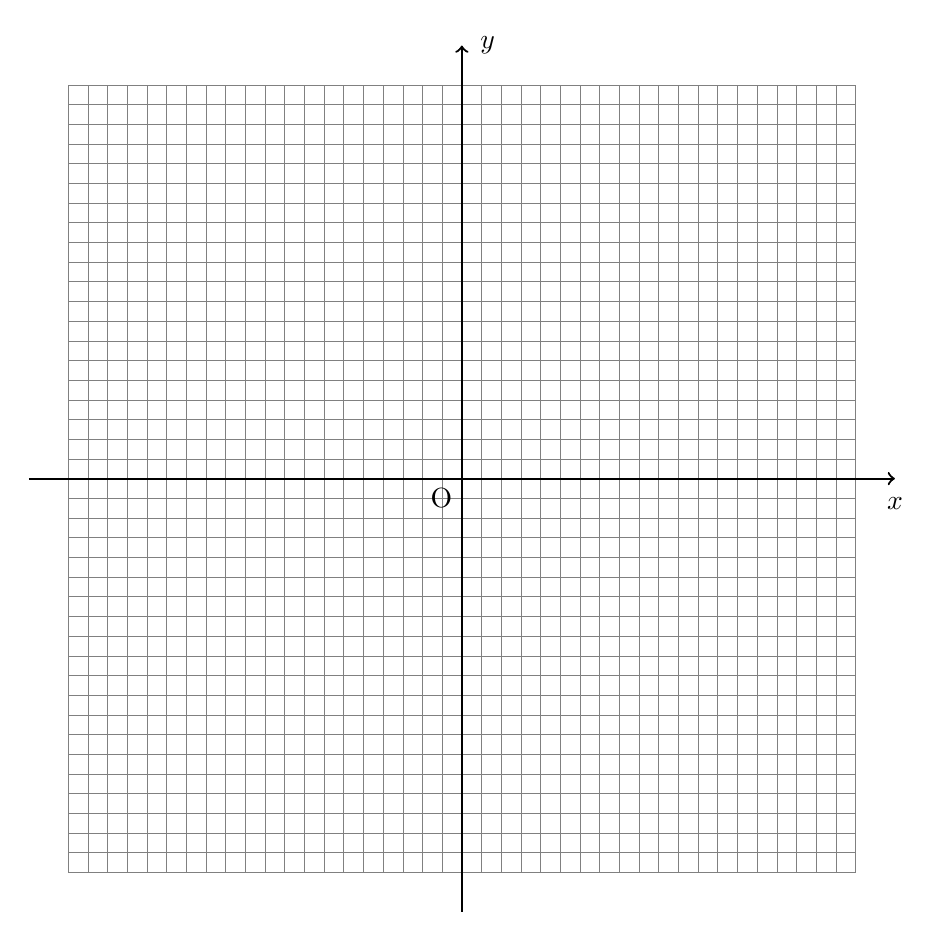
\begin{tikzpicture}
	\draw[help lines, step=0.25] (0,0) grid (10,10);
	\draw (5,5) node[below left]{O};
	\draw[thick, ->] (-0.5,5)--(10.5,5) node[below=3.0] {$x$};
	\draw[thick, ->] (5,-0.5)--(5,10.5) node[right=3.0] {$y$};
	\end{tikzpicture}
	\caption{代数関数のグラフの図示}
	\label{fig:algebraicFunction}
\end{figure}
\clearpage

\section{指数関数}
多項式関数は,$x$を変数,$n$をパラメータとして,$f(x) = x^n$という形を取っていた.このとき,$x$を\textbf{底},$n$を\textbf{指数}と呼ぶ.つまり,多項式関数は,指数をパラメータとして先に決め,底を変数として,ある集合の中の要素を取り得るよう定めたもの,と考えることができる.

指数関数は,この多項式関数における変数とパラメータの役割を交換し,底をパラメータとして先に決め,指数を変数として,ある集合の中の要素を取り得るよう定める.つまり,$a$を底,$x$を指数として,$f(x) = a^x$を考える.
この関数の性質を考える上で,基本となる考え方が,自然数においての指数法則である.指数法則が成り立つ範囲を実数の範囲まで拡張したとき,特定の数の集合を一対一の関係で結びつける写像が存在する.それこそが,指数関数であることを,この節では見ていく.

\begin{definition}[自然数における指数法則]
	\label{def:exponentialLawN}%
	$a, b$を$0$を除いた実数,$n, m$を自然数(ただし,$n > m$)とする.このとき,
	\begin{enumerate}[1.]
		\item $a^na^m = a^{n+m}$
		\item $a^n / a^m = a^{n-m}$
		\item $\left(a^n\right)^m = a^{nm} = \left(a^m\right)^n$
		\item $\left(ab\right)^n = a^nb^n$
	\end{enumerate}
	が成り立ち,このことを,指数法則と呼ぶ.
\end{definition}
\begin{example*}
	$2^2\cdot 2^3$は,$(2\cdot2)\cdot(2\cdot2\cdot2)$であるため,$2^5$となる.つまり,$2^2\cdot2^3 = 2^{2+3} = 2^5$である.
	$2^3/2^2$は,$(2\cdot2\cdot2)/(2\cdot2)$であるため,$2^1$となる.つまり,$2^3/2^2 = 2^{3-2} = 2^1$である.
	$\left(2^2\right)^3$は,$(2\cdot2)\cdot(2\cdot2)\cdot(2\cdot2)$であるため,$2^6$となる.つまり,$\left(2^2\right)^3 = 2^{2\cdot3} = 2^6$である.
\end{example*}

定義\ref{def:exponentialLawN}において,$n > m$を仮定した.しかし,$m$を自然数として,$a^0 = 1$,$a^{-m} = 1/a^m$と定義することによって,指数法則は,整数の範囲まで拡張される.

\begin{definition}[整数における指数法則]
	\label{def:exponentialLawZ}%
	$a, b$を$0$を除いた実数,$n, m$を整数とする.このとき,
	\begin{enumerate}[1.]
		\item $a^n\cdot a^m = a^{n+m}$
		%\item $a^n / a^m = a^{n-m}$
		\item $\left(a^n\right)^m = a^{nm} = \left(a^m\right)^n$
		\item $\left(ab\right)^n = a^nb^n$
	\end{enumerate}
	が成り立ち,このことを,指数法則と呼ぶ.
\end{definition}

また,$n$を整数,$m$を自然数として,$r = n/m$となる有理数を考える.このとき,$a$を正の実数とし,$a^r = a^{n/m} = \left(\sqrt[m]{a}\right)^n$と定義すれば,指数法則は,有理数の範囲まで拡張される\footnotemark[1].また,実数$x$は,$r < x < s$という不等式が成り立つように有理数$r, s$を選んで表すことができる.$r, s$は,$x$に有理数の範囲でいくらでも近づけていけるため,$a$を正の実数とすれば,$a^x$の値を,$a^r, a^s$を用いて評価できる.このとき,指数法則は,実数の範囲まで拡張され,実数全体の集合$\mathbb{R}$と,正の実数全体の集合$\mathbb{R}_{>0}$を一対一の関係で結びつける\footnotemark[2].この関係を,$a$を底とする指数関数と呼ぶ.
\footnotetext[1]{指数の取り得る範囲は拡張されるが,代わりに,底の取り得る範囲は縮小する.このような場合,基本的に変数の取り得る範囲を拡張することが優先される.}
\footnotetext[2]{この関係は,全域的であるため,写像である.さらに,終域が数の集合であるため,関数でもある.直積集合$\mathbb{R}\times\mathbb{R}$の部分集合である関係$R$が,指数法則が成り立つ写像として定義されていく味わい深さを感じ取って貰えれば幸いである.}
% 有理数の指数を,冪根(累乗根)と紐づける.

\begin{definition}[実数における指数法則]
	\label{def:exponentialLawR}%
	$a, b$を正の実数,$x, y$を実数とする.このとき,
	\begin{enumerate}[1.]
		\item $a^x\cdot a^y = a^{x+y}$
		%\item $a^x / a^y = a^{x-y}$
		\item $\left(a^x\right)^y = a^{xy} = \left(a^y\right)^x$
		\item $\left(ab\right)^x = a^xb^x$
	\end{enumerate}
	が成り立ち,このことを,指数法則と呼ぶ.
\end{definition}
\begin{definition}[指数関数]
	$1$を除いた正の実数$a$が与えられているとき,関数$f : \mathbb{R} \rightarrow \mathbb{R}; x \mapsto a^x$のことを,$a$を底とする\textbf{指数関数}と呼ぶ.$x$における$f$の値が,$a^x$であるため,これを用いて$y = a^x$や$f(x) = a^x$と表記される.
\end{definition}
\begin{rem*}
	指数関数$f(x) = a^x$の像$\im f$は,正の実数全体の集合$\mathbb{R}_{>0}$である.
\end{rem*}
\begin{example*}
	$a > 1$,$0 < a < 1$の場合における指数関数のグラフを示したものが,図\ref{fig:exponentialFunction}である.$a > 1$の例として,$y = 2^x$を,$0 < a< 1$の例として,$y=0.5^x$を選んだ.
	
	\begin{figure}[!h]
		\centering
		\begin{tikzpicture}
			\begin{axis}[
				clip = true,
				clip mode=individual,
				domain = -2.5:2.5,
				restrict y to domain=-0.5:4.5,
				axis lines=center,
				xlabel=$x$,
				xlabel style={at=(current axis.right of origin), anchor=west},
				ylabel=$y$,
				xmin=-2.5,
				xmax=2.5,
				enlarge x limits={rel=0.07},
				ymin=-0.5,
				ymax=4.5,
				enlarge y limits={rel=0.13}				
			]
			\node[below left] at (axis cs:0,0) {O};
			\addplot[samples=100]{2^x} node[above, pos=1]{$y = 2^x$};
			\addplot[samples=100]{0.5^x} node[above,pos=0]{$y = 0.5^x$};
			\end{axis}
		\end{tikzpicture}
		\caption{指数関数のグラフの図示}
		\label{fig:exponentialFunction}
	\end{figure}
\end{example*}

\begin{definition}[単調関数]
	実数の部分集合である開区間$(a, b)$で定義されている関数$f(x)$について,一定の条件を満たすことで,性質が定義される.ここで,$s, t$は,$(a, b)$に属する実数とする.
	\begin{align*}
		\text{$f(x)$は,$(a, b)$で\textbf{単調増加}である.} &\Leftrightarrow \text{$s < t$ならば,$f(s) < f(t)$である.} \\
		\text{$f(x)$は,$(a, b)$で\textbf{単調非減少}である.} &\Leftrightarrow \text{$s < t$ならば,$f(s) \leq f(t)$である.} \\
		\text{$f(x)$は,$(a, b)$で\textbf{単調減少}である.} &\Leftrightarrow \text{$s < t$ならば,$f(s) > f(t)$である.} \\
		\text{$f(x)$は,$(a, b)$で\textbf{単調非増加}である.} &\Leftrightarrow \text{$s < t$ならば,$f(s) \geq f(t)$である.} 
	\end{align*}
\end{definition}
\begin{rem*}
	「単調増加」のことを,「狭義単調増加」と呼び,「単調非減少」のことを「広義単調増加」と呼ぶこともある.同様に,「単調減少」のことを,「狭義単調減少」と呼び,「単調非増加」のことを「広義単調減少」と呼ぶこともある.
\end{rem*}
\begin{example*}
	指数関数$y = a^x$は,$a > 1$のとき,単調増加であり,$0 < a < 1$のとき,単調減少である.
\end{example*}

\newpage
\section{対数関数}
指数関数$y = a^x$では,$x$を変数とし,それに伴って変化する値である$y$を求めた.
この節では,$y$を変数とし,それに伴って変化する$x$を求めるための新しい関数を定義する.
そのために,定義\ref{def:binaryRelation}で学んだ関係の概念に付随する,逆関係を導入する.その後,写像や関数に対応する逆写像,逆関数を定義し,指数関数の逆関数として,対数関数を定義することにする.
% 対数関数とは,「底$a$を何乗したら値$y$になるのか」を考えるための関数である.
% 指数関数$y = a^x$は,単射であるため,正の実数$M$に対して,$a^x = M$となる実数$x$が一意的に定まる.

\begin{definition}[逆関係]
	集合$A, B$間の二項関係$R$における\textbf{逆関係}$R^{-1}$とは,
	\[
		R^{-1} = \set{(b,a) \mid (a,b)\in R}
	\]
	と定義される集合のことである.
\end{definition}
\begin{definition}[逆写像・逆関数]
	写像あるいは関数$f$について,$f$は二項関係とみなせるため,その逆関係$f^{-1}$が定まる.
	この$f^{-1}$が,写像あるいは関数の定義を満たした場合,$f^{-1}$を,$f$の\textbf{逆写像}あるいは\textbf{逆関数}と呼ぶ.
\end{definition}
\begin{theorem}
	関係$R$が,一対一ならば,逆関係$R^{-1}$も,一対一である.
\end{theorem}
\begin{theorem}
	\label{thm:inverseMapping1}%
	写像$f$が,全単射ならば,逆写像$f^{-1}$が存在し,$f^{-1}$も全単射である.
\end{theorem}
\begin{rem*}
	このとき,$\dom f = \cod f^{-1}$であり,$\cod f = \dom f^{-1}$である.つまり,写像$f : A \rightarrow B$に対して,逆写像$f^{-1} : B \rightarrow A$である.
\end{rem*}
\begin{theorem}
	\label{thm:inverseMapping2}%
	写像あるいは関数$f$が,単射であるとき,写像あるいは関数$g: \dom f \rightarrow \im f$は,全単射である.
\end{theorem}
% % % 関数$f$と逆関数$f^{-1}$に対して,常に$f(f^{-1}(x)) = f^{-1}(f(x)) = x$が成り立つ.

指数関数$f(x) = a^x$は,単射であるため,定理\ref{thm:inverseMapping2}より,関数$g : \mathbb{R} \rightarrow \mathbb{R}_{>0}; x \mapsto a^x$は,全単射となる.このとき,定理\ref{thm:inverseMapping1}より,逆写像$g^{-1} : \mathbb{R}_{>0} \rightarrow \mathbb{R}$が存在する.この逆写像は,終域が数の集合であるため,逆関数でもある.
\begin{definition}[対数関数]
	$a$を$1$を除いた正の実数とする.関数$f : \mathbb{R} \rightarrow \mathbb{R}_{>0}; x \mapsto y = a^x$について,逆関数$f^{-1} : \mathbb{R}_{>0} \rightarrow \mathbb{R}; y \mapsto x$を,$a$を底とする\textbf{対数関数}と呼ぶ.このとき,$y$における$f^{-1}$の値を$x = \log_a y$と表記する.
\end{definition}
\begin{rem*}
	逆関数のままでは,扱いにくいため,素直に関数$f : \mathbb{R}_{>0} \rightarrow \mathbb{R}; x \mapsto \log_a x$と書かれることが多い.これは,対数関数の定義中で出てくる文字を置き換えただけである.
\end{rem*}
\begin{rem*}
	平たく言えば,対数関数とは,「底$a$を何乗したら$x$になるのか」を考えるための関数である.すなわち,$2^3 = 8$であるため,$\log_2 8 = 3$である.
\end{rem*}
\begin{rem*}
	定義より明らかに,$\log_a a^x = x$であり,$a^{\log_a y} = y$である.すなわち,
	\begin{align*}
		\log_a a &= \log_a a^1 = 1 \\
		\log_a 1 &= \log_a a^0 = 0
	\end{align*}
	となる.
\end{rem*}
\begin{rem*}
	対数関数$y = \log_a x$は,$a > 1$のとき,単調増加であり,$0 < a < 1$のとき,単調減少である.
\end{rem*}

\begin{theorem}
	指数法則から,以下に示す対数関数の各種性質が導かれる.ここで,$a, b$は$1$を除いた正の実数,$x, y$は正の実数,$r$は実数とする.
	\begin{enumerate}[itemsep=2ex, label*=\arabic*.]
		\item $\log_a xy = \log_a x + \log_a y$
		\item $\displaystyle \log_a \frac{x}{y} = \log_a x - \log_a y$
		\item $\log_a x^r = r\log_a x$
		\item $\displaystyle \log_a x = \frac{\log_b x}{\log_b a}$
	\end{enumerate}
\end{theorem}

図\ref{fig:logarithmicFunction}に,$a > 1$,$0 < a < 1$の場合における対数関数のグラフを示す.$a > 1$の例として,$y = \log_2 x$を,$0 < a< 1$の例として,$y=\log_{1/2} x$を選んだ.また,図\ref{fig:inverseFunction}に,指数関数$y = 2^x$のグラフと対数関数$y = \log_2 x$のグラフを示した.一般的に,ある関数$f$のグラフとその逆関数$f^{-1}$のグラフは,直線$y = x$に関して対称となる.

\begin{figure}[!h]
	\centering
	\begin{tikzpicture}
	\begin{axis}[
	clip = true,
	clip mode=individual,
	domain = 0.01:4.50,
	restrict y to domain=-4.0:4.0,
	axis lines=center,
	xlabel=$x$,
	xlabel style={at=(current axis.right of origin), anchor=west},
	ylabel=$y$,
	ylabel style={at=(current axis.above origin), anchor=south},
	xmin=-0.5,
	xmax=4.5,
	enlarge x limits={rel=0.07},
	ymin=-3.0,
	ymax=3.0,
	enlarge y limits={rel=0.13}				
	]
	\node[below left] at (axis cs:0,0) {O};
	\addplot[samples=200]{ln(x)/ln(2)} node[above left, pos=1]{$y = \log_2 x$};
	\addplot[samples=200]{ln(x)/ln(0.5)} node[below left,pos=1]{$y = \log_{1/2} x$};
	\end{axis}
	\end{tikzpicture}
	\caption{対数関数のグラフの図示}
	\label{fig:logarithmicFunction}
\end{figure}

\begin{figure}[!h]
	\centering
	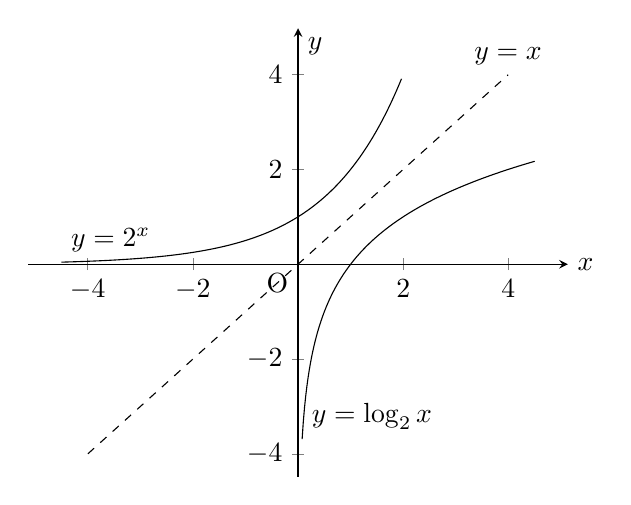
\begin{tikzpicture}
	\begin{axis}[
	clip = true,
	clip mode=individual,
	%domain = 0.01:4.50,
	restrict y to domain=-4.0:4.0,
	axis lines=center,
	xlabel=$x$,
	xlabel style={at=(current axis.right of origin), anchor=west},
	ylabel=$y$,
	xmin=-4.5,
	xmax=4.5,
	enlarge x limits={rel=0.07},
	ymin=-3.5,
	ymax=4.0,
	enlarge y limits={rel=0.13}				
	]
	\node[below left] at (axis cs:0,0) {O};
	\addplot[domain = -4.50:4.50, samples=200]{2^x} node[above right, pos=0]{$y = 2^x$};
	\addplot[domain =  0.01:4.50, samples=200]{ln(x)/ln(2)} node[above right, pos=0]{$y = \log_2 x$};
	\addplot[dashed, samples=200]{x} node[above,pos=1]{$y = x$};
	\end{axis}
	\end{tikzpicture}
	\caption{指数関数と対数関数のグラフの図示}
	\label{fig:inverseFunction}
\end{figure}

\clearpage
\section{三角関数}
自然現象をはじめとする様々な現象を観察すると,おおまかに比例関係・指数増加・周期変化の組み合わせであることが確認できる.
つまり,とある現象をモデル化する(数式で記述する)ためには,それら一つ一つに数式を対応させなければならない.
例えば,比例関係は代数関数$f(x) = ax+b$と,指数増加は指数関数$f(x) = Ca^x$と,それぞれ対応づけることができる.
この節では,周期変化を記述するための関数として,三角関数を定義し,その性質を見ていく.

% 指数関数・対数関数は,全域にわたって単調に増減のどちらかを行う関数であった.関数の中には,周期的に増減を繰り返すものを考えることができる.この節では,周期的に変化を繰り返す関数の代表例として,三角関数を学ぶ.
% 三角関数は,定義のされ方から円と関わりが深い.また,その定義から,三角比の値を取ることが分かる.
% 自然現象をモデル化するに当たって,比例関係・指数増加・周期変化を記述する必要がある.
% そのため,それぞれに代数関数・指数関数・三角関数が対応し,自然現象のモデルを用いて変化を予測するために,関数の変化を考える必要があるということを改めて認識して欲しい.

\begin{definition}[周期関数]
	関数$f$の始域の要素$T$に対して,常に$f(x) = f(x + T)$が成り立つとき,関数$f$は\textbf{周期的}であるといい,$f$を\textbf{周期関数}と呼ぶ.また,関数を周期的にするような$T$のうち,絶対値が最小かつ正のものを\textbf{周期}と呼ぶ.
\end{definition}

\begin{definition}[単位円]
	関係$R = \set{(x,y) \mid x^2+y^2 = 1}$のグラフを,\textbf{単位円}と呼ぶ.
\end{definition}
\begin{definition}[動径]
	ある半直線OAが与えられているとき,半直線OAを,点Oを中心に$\theta$だけ回転させた半直線OPのことを\textbf{動径}と呼ぶ.また,半直線OAのことを\textbf{始線}と呼ぶ.
\end{definition}
\begin{rem*}
	$\theta$が正のとき,反時計回りに回転し,$\theta$が負のとき,時計回りに回転するものと定義する.
\end{rem*}
\begin{rem*}
	円と$x$軸との交点のうち,$x$座標が正のものを点Aとして,原点Oから伸びる半直線OAを始線とするとき,円と動径の交点が点Pである.
\end{rem*}
\begin{definition}[弧度法]
	動径OPと単位円周上の点$\mathrm{A} = (1, 0)$が与えられているとき,弧APの長さが1になるような動径の角度$\theta$を$\SI{1}{\radian}$と定義する.この角度の決め方を,弧度法という.弧度法に対して,円周一周分の角度を$\SI{360}{\degree}$と定義する方法を,度数法という.
\end{definition}
% % % 長さの定義とか,円周の定義とかしてない!
\begin{example*}
	$\SI{360}{\degree} = \SI{2\pi}{\radian}$である.
\end{example*}

\begin{definition}[三角関数]
	\label{def:trigonometricFunction}%
	単位円周上の点$\mathrm{A} = (1, 0)$を用いて始線OAを定める.
	このとき,角度$\theta$を決めることによって,単位円と動径の交点Pの座標は一意的に決定できる.
	また,動径の定義より,角度の変化に伴う座標の変化は周期的になる.
	ここで,角度$\theta$と点Pの$x$座標の関係$\theta \mapsto x$,角度$\theta$と点Pの$y$座標の関係$\theta \mapsto y$は,それぞれ写像の定義を満たす.
	そのため,$x = f(\theta) = \cos(\theta)$,$y = g(\theta) = \sin(\theta)$と定義すると,
	写像$f, g$は,周期$2\pi$の周期関数$f, g : \mathbb{R} \rightarrow [-1, 1]$となる.
	
	また,動径OPと直線$x=1$との交点をTとすると,点Tの$y$座標は,すべての実数を取り得る.
	この関係$\theta \mapsto y$も写像の定義を満たすため,$y = h(\theta) = \tan(\theta)$と定義すると,
	写像$h$は,周期$\pi$の周期関数$h : \mathbb{R}\setminus\set{\pi/2 + n\pi \mid n \in \mathbb{Z}} \rightarrow \mathbb{R}$となる.
	
	図\ref{fig:unitCircle}は,三角関数の定義を図示したものである.
\end{definition}

\begin{figure}[!h]
	\centering
	\begin{tikzpicture}
	\begin{axis}[
	width=10cm,
	height=10cm,
	clip = true,
	clip mode=individual,
	%domain = 0.01:4.50,
	%restrict y to domain=-1.0:1.0,
	axis lines=center,
	xlabel=$x$,
	xlabel style={at=(current axis.right of origin), anchor=west},
	ylabel=$y$,
	xmin=-1.0,
	xmax=1.0,
	enlarge x limits={rel=0.10},
	ymin=-1.0,
	ymax=1.0,
	enlarge y limits={rel=0.10},
	xtick distance=1,
	x tick label style={anchor=north west},
	ytick distance=1
	]
	\node[below left] at (axis cs:0,0) {O};
	\addplot[samples=200, domain = 0:2*pi, name path=circle]( {cos(deg(x))}, {sin(deg(x))} );
	\node[above left] at (axis cs:1,0) {A};
	
	\draw[name path=op] (axis cs:0,0) -- ++(45:5.5cm);
	\fill[name intersections={of=circle and op}] (intersection-1) circle (0pt) node[anchor=west] {P=$(\cos\theta, \sin\theta)$};
	
	\coordinate (O) at (axis cs:0,0);
	\coordinate (A) at (axis cs:1,0);
	\draw pic["$\theta$",draw=black, ->, thick, angle eccentricity=1.2, angle radius=1cm] {angle=A--O--intersection-1};
	
	\draw[name path=ot] (axis cs:1,-1.3) -- (axis cs:1,1.3);
	\fill[name intersections={of=op and ot}] (intersection-1) circle (0pt) node[anchor=west] {T=$(1, \tan\theta)$};
	\end{axis}	
	\end{tikzpicture}
	\caption{三角関数の定義}
	\label{fig:unitCircle}
\end{figure}

\begin{rem*}
	括弧の中身が複雑でない場合,$\sin\theta, \cos\theta, \tan\theta$のように括弧が省略されて書かれることが多い.
\end{rem*}
\begin{rem*}
	円と動径の交点Pの座標を$(x,y)$,線分OPの長さを$r$とすると,
	\begin{align*}
		\sin\theta &= \frac{y}{r} & \cos\theta &= \frac{x}{r} & \tan\theta &= \frac{y}{x} \\[5pt]
		\csc\theta &= \frac{r}{y} & \sec\theta &= \frac{r}{x} & \cot\theta &= \frac{x}{y}
	\end{align*}
	のように$x, y, r$の組み合わせ6種類を考えることができる.これらは,定義\ref{def:trigonometricFunction}の別な形であり,これら6つの関数のことを\textbf{三角関数}と呼ぶ.
\end{rem*}
\begin{example*}
	$xy$平面の,原点から見て右上・左上・左下・右下の領域を,それぞれ第一象限・第二象限・第三象限・第四象限と呼ぶ.
	定義より,三角関数の値がとる符号は,動径がどの象限に入るかによって定まり,それを図示したものが,図\ref{fig:triFuncSign}である.
	
	\vspace*{5cm}
	\begin{figure}[!h]
		\centering
		\caption{三角関数の値の符号}
		\label{fig:triFuncSign}
	\end{figure}
\end{example*}
\begin{example*}
	特徴的な三角関数の値を表\ref{table:triFuncValue}に示す.他の角度における三角関数の値は,動径がどの象限にあるのか,表に載っている角度とどのような関係にあるのか,などいくつかの条件をもとに考えるとよい.
	
	\begin{table}[!h]
		\centering
		\caption{三角関数の代表値}
		\label{table:triFuncValue}
		\begin{tabular}{c|ccccc}
			$\theta$ & 0 & $\pi/6$ & $\pi/4$ & $\pi/3$ & $\pi/2$ \\
			\hline
			$\sin\theta$ & 0 & $1/2$ & $1/\sqrt{2}$ & $\sqrt{3}/2$ & 1 \\
			\hline
			$\cos\theta$ & 1 & $\sqrt{3}/2$ & $1/\sqrt{2}$ & $1/2$ & 0 \\
			\hline
			$\tan\theta$ & 0 & $1/\sqrt{3}$ & 1 & $\sqrt{3}$ & -
		\end{tabular}
	\end{table}
\end{example*}

\begin{theorem}[三角関数の相互関係]
	三角関数の定義より,以下の相互関係が導かれる.
	\begin{enumerate}[itemsep=2ex, label*=\arabic*.]
		\item $\displaystyle \tan\theta = \frac{\sin\theta}{\cos\theta}$
		\item $\displaystyle \sin^2\theta + \cos^2\theta = 1$
		\item $\displaystyle \tan^2\theta + 1 = \frac{1}{\cos^2\theta} = \sec^2\theta$
	\end{enumerate}
\end{theorem}

三角関数のグラフを,図\ref{fig:triFunc}に示す.

\begin{figure}[!h]
	\centering
	\begin{subfigure}[t]{.5\textwidth}
		\begin{tikzpicture}
		\begin{axis}[
		width=\textwidth,
		axis lines=center,
		xlabel=$\theta$,
		xlabel style={at=(current axis.right of origin), anchor=west},
		ylabel=$y$,
		xmin=-2.0,
		xmax=7.0,
		ymin=-1.0,
		ymax=1.0,
		enlarge y limits={rel=0.10},
		xtick={-1.57, 1.57, 3.14, 4.71, 6.28},
		xticklabels={$-\pi/2$,$\pi/2$, $\pi$, $3\pi/2$, $2\pi$},
		x tick label style={anchor=north},
		ytick distance=1
		]
		\node[below left] at (axis cs:0,0) {O};
		\addplot[samples=200, domain = -2:7]{sin(deg(x))};
		\end{axis}	
		\end{tikzpicture}
		\caption{$\sin\theta$のグラフ}
	\end{subfigure}%
	\begin{subfigure}[t]{.5\textwidth}
		\begin{tikzpicture}
		\begin{axis}[
		width=\textwidth,
		axis lines=center,
		xlabel=$\theta$,
		xlabel style={at=(current axis.right of origin), anchor=west},
		ylabel=$y$,
		xmin=-2.0,
		xmax=7.0,
		ymin=-1.0,
		ymax=1.0,
		enlarge y limits={rel=0.10},
		xtick={-1.57, 1.57, 3.14, 4.71, 6.28},
		xticklabels={$-\pi/2$,$\pi/2$, $\pi$, $3\pi/2$, $2\pi$},
		x tick label style={anchor=north},
		ytick distance=1
		]
		\node[below left] at (axis cs:0,0) {O};
		\addplot[samples=200, domain = -2:7]{cos(deg(x))};
		\end{axis}	
		\end{tikzpicture}
		\caption{$\cos\theta$のグラフ}
	\end{subfigure}\\%
	\begin{subfigure}[t]{.5\textwidth}
		\begin{tikzpicture}
		\begin{axis}[
		width=\textwidth,
		axis lines=center,
		xlabel=$\theta$,
		xlabel style={at=(current axis.right of origin), anchor=west},
		ylabel=$y$,
		xmin=-2.0,
		xmax=7.0,
		ymin=-1.0,
		ymax=1.0,
		enlarge y limits={rel=0.10},
		xtick={-1.57, 1.57, 3.14, 4.71, 6.28},
		xticklabels={$-\pi/2$,$\pi/2$, $\pi$, $3\pi/2$, $2\pi$},
		x tick label style={anchor=north},
		ytick distance=1
		]
		\node[below left] at (axis cs:0,0) {O};
		\addplot[samples=200, domain = -4*pi/3:-2*pi/3]{tan(deg(x))};
		\addplot[samples=200, domain = -pi/3:pi/3]{tan(deg(x))};
		\addplot[samples=200, domain = 2*pi/3:4*pi/3]{tan(deg(x))};
		\addplot[samples=200, domain = 5*pi/3:7*pi/3]{tan(deg(x))};
		\end{axis}	
		\end{tikzpicture}
		\caption{$\tan\theta$のグラフ}
	\end{subfigure}
	\caption{三角関数のグラフ}
	\label{fig:triFunc}
\end{figure}

\clearpage
\begin{definition}[偶関数]
	関数$f$について,常に$f(-x) = f(x)$が成り立つとき,関数$f$を\textbf{偶関数}と呼ぶ.このとき,グラフは$y$軸に関して対称となる.
\end{definition}
\begin{definition}[奇関数]
	関数$f$について,常に$f(-x) = -f(x)$が成り立つとき,関数$f$を\textbf{奇関数}と呼ぶ.このとき,グラフは原点に関して対称となる.
\end{definition}
\begin{example*}
	関数$f(\theta) = \cos\theta$は,偶関数である.関数$f(\theta) = \sin\theta$,$f(\theta) = \tan\theta$は,奇関数である.
\end{example*}

\begin{theorem}[加法定理]
	実数$\alpha, \beta$について,以下の等式が成り立つ.
	\begin{enumerate}[itemsep=2ex, label*=\arabic*.]
		\item $\displaystyle \sin(\alpha+\beta) = \sin\alpha\cos\beta + \cos\alpha\sin\beta$
		\item $\displaystyle \cos(\alpha+\beta) = \cos\alpha\cos\beta - \sin\alpha\sin\beta$
	\end{enumerate}
\end{theorem}
\begin{example*}
	三角関数の加法定理を第一象限内で図示したものが,図\ref{fig:triAdditionTheorem}である.
	
	\begin{figure}[!h]
		\centering
		\begin{tikzpicture}
		\coordinate (O) at (0,0);
		\coordinate (A) at (3,0);
		\coordinate (B) at (3,1.25);
		\coordinate (C) at (3,4.25);
		\coordinate (P) at (1.75,4.25);
		
		\node[below left] at (O) {O};
		\node[below right] at (A) {A};
		\node[right] at (B) {B};
		\node[above right] at (C) {C};
		\node[above left] at (P) {P};

		\draw[name path=oa] (O) -- (A);
		\draw[name path=ob] (O) -- (B);
		\draw[name path=op] (O) -- (P) node at ($(O)!0.5!(P)$) [left]{1};
		\draw[name path=ab] (A) -- (B);
		\draw[name path=bc] (B) -- (C);
		\draw[name path=bp] (B) -- (P);
		\draw[name path=pc] (P) -- (C);

		\draw[thick, black] ($(A)!8pt!(O)$)--($(A)!8pt!(B)!8pt!90:(B)$)--($(A)!8pt!(B)$);
		\draw[thick, black] ($(B)!8pt!(O)$)--($(B)!8pt!(P)!8pt!90:(P)$)--($(B)!8pt!(P)$);
		\draw[thick, black] ($(C)!8pt!(B)$)--($(C)!8pt!(P)!8pt!90:(P)$)--($(C)!8pt!(P)$);

		\draw pic["$\alpha$",draw=black, -, thick, angle eccentricity=1.2, angle radius=1cm] {angle=A--O--B};
		\draw pic["$\beta$",draw=black, -, thick, angle eccentricity=1.2, angle radius=1.2cm] {angle=B--O--P};
		\draw pic["$\alpha$",draw=black, -, thick, angle eccentricity=1.2, angle radius=1cm] {angle=C--B--P};
		\end{tikzpicture}
		\caption{加法定理の幾何学的意味}
		\label{fig:triAdditionTheorem}
	\end{figure}
\end{example*}
% % % 倍角・半角の公式の導出や和積・積和の公式の導出
% % % 例題を入れる

\clearpage
\section{逆三角関数}
この節では,三角関数の逆関数として,逆三角関数を定義する.
そもそも三角関数は,周期関数であるため,単射ではなく,逆関数を作ることができない.そのため,0を含むような1周期を始域とする制限された三角関数を考えることで,単射とすることができ,逆三角関数を定義することができるようになる.
 
\begin{definition}[逆三角関数]
	制限された三角関数を,
	\begin{align*}
		\sin &: [-\pi/2, \pi/2] \rightarrow [-1, 1] \\
		\cos &: [0, \pi] \rightarrow [-1, 1] \\
		\tan &: (-\pi/2, \pi/2) \rightarrow \mathbb{R}
	\end{align*}
	とする.このとき.それぞれの逆三角関数を,
	\begin{align*}
		\arcsin &: [-1, 1] \rightarrow [-\pi/2, \pi/2] \\
		\arccos &: [-1, 1] \rightarrow [0, \pi] \\
		\arctan &: \mathbb{R} \rightarrow (-\pi/2, \pi/2)
	\end{align*}
	と定義する.
\end{definition}
\begin{rem*}
	逆三角関数$\arcsin, \arccos, \arctan$のことを,$\sin^{-1}, \cos^{-1}, \tan^{-1}$と表記することもある.この表記は,$x^{-1}$のような逆数としての$-1$との混乱を生む可能性があるため,この文書では使わない.
\end{rem*}
\begin{example*}
	$\sin(\pi/4) = 1/\sqrt{2}$より,$\arcsin(1/\sqrt{2}) = \pi/4$である.
\end{example*}
\begin{example*}
	指数関数・対数関数と同様に,逆関数の関係にあるため,$\sin(\arcsin(x)) = x$である.
\end{example*}

逆三角関数のグラフを,図\ref{fig:invTriFunc}に示す.$f(x) = \arcsin x$と$f(x) = \arctan x$は,単調増加であり,$f(x) = \arccos x$は,単調減少である.

\begin{figure}[!h]
	\centering
	\begin{subfigure}[t]{.5\textwidth}
		\begin{tikzpicture}
		\begin{axis}[
		width=\textwidth,
		axis lines=center,
		xlabel=$x$,
		xlabel style={at=(current axis.right of origin), anchor=west},
		ylabel=$y$,
		xmin=-1.0,
		xmax=1.0,
		ymin=-2.0,
		ymax=2.0,
		enlarge y limits={rel=0.10},
		xtick distance=1,
		ytick={-1.57, 1.57},
		yticklabels={$-\pi/2$,$\pi/2$},
		]
		\node[below left] at (axis cs:0,0) {O};
		\addplot[samples=200, domain = -1:1]{rad(asin(x))};
		\end{axis}	
		\end{tikzpicture}
		\caption{$\arcsin x$のグラフ}
	\end{subfigure}%
	\begin{subfigure}[t]{.5\textwidth}
		\begin{tikzpicture}
		\begin{axis}[
		width=\textwidth,
		axis lines=center,
		xlabel=$x$,
		xlabel style={at=(current axis.right of origin), anchor=west},
		ylabel=$y$,
		xmin=-1.0,
		xmax=1.0,
		ymin=-0.5,
		ymax=3.5,
		enlarge y limits={rel=0.10},
		xtick distance=1,
		ytick={1.57, 3.14},
		yticklabels={$\pi/2$,$\pi$},
		]
		\node[below left] at (axis cs:0,0) {O};
		\addplot[samples=200, domain = -1:1]{rad(acos(x))};
		\end{axis}	
		\end{tikzpicture}
		\caption{$\arccos x$のグラフ}
	\end{subfigure}\\%
	\begin{subfigure}[t]{.5\textwidth}
		\begin{tikzpicture}
		\begin{axis}[
		width=\textwidth,
		axis lines=center,
		xlabel=$x$,
		xlabel style={at=(current axis.right of origin), anchor=west},
		ylabel=$y$,
		xmin=-4.0,
		xmax=4.0,
		ymin=-2.0,
		ymax=2.0,
		enlarge y limits={rel=0.10},
		xtick distance=1,
		ytick={-1.57, 1.57},
		yticklabels={$-\pi/2$,$\pi/2$},
		]
		\node[below left] at (axis cs:0,0) {O};
		\addplot[samples=200, domain = -4:4]{rad(atan(x))};
		\end{axis}	
		\end{tikzpicture}
		\caption{$\arctan x$のグラフ}
	\end{subfigure}
	\caption{逆三角関数のグラフ}
	\label{fig:invTriFunc}
\end{figure}
